\section{Durchführung}
\label{sec:Durchführung}

Auf der Arbeitsfläche stehen ein analoges Oszilloskop und eine Leiterplatte, sowie ein Tastkopf mit Erdungsklemme. Der Tastkopf hat einen integrierten Spannungsteiler, der über einen Schalter aktiviert werden kann. Ausgeschaltet hat der Tastkopf eine Spannungteilung von 1, während dieser angeschaltet die Spannung mit $\frac{1}{10}$ multipliziert bzw. mit 10 dividiert.

\subsection{Das Oszilloskop}

\begin{figure}[htbp]
	\begin{minipage}[c]{0.55\linewidth}
		Der Versuch wird mit dem analogen Oszilloskop 35 MHz Analog Oscilloscope HM303-6 der Marke Hameg Instruments durchgeführt. Das verwendete Oszilloskop ist ein Elektronenstrahl-Oszilloskop zur zeitabhängigen Darstellung elektrischer Spannungsverläufe $U(t)$.
		
		In einer Kathodenstrahlröhre emittiert eine Kathode Elektronen. Diese werden durch Elektroden gebündelt und durch eine Anodenspannung in Richtung eines Phosphorleuchtschirms beschleunigt, wo sie beim Auftreffen einen sichtbaren, nicht unbedingt statischen Lichtpunkt erzeugen. Dabei kann dieses Licht weiterhin durch Einstellungen am Oszilloskop beeinflusst werden.\cite{V300}
		
		\subsubsection{Relevante Bedienelemente}
		Die Bedienfläche des Oszilloskops unterteilt sich in vier für diesen Versuch wichtige Funktionsbereiche.
	\end{minipage}%
	\hfill
	\begin{minipage}[c]{0.4\linewidth}
		\centering
		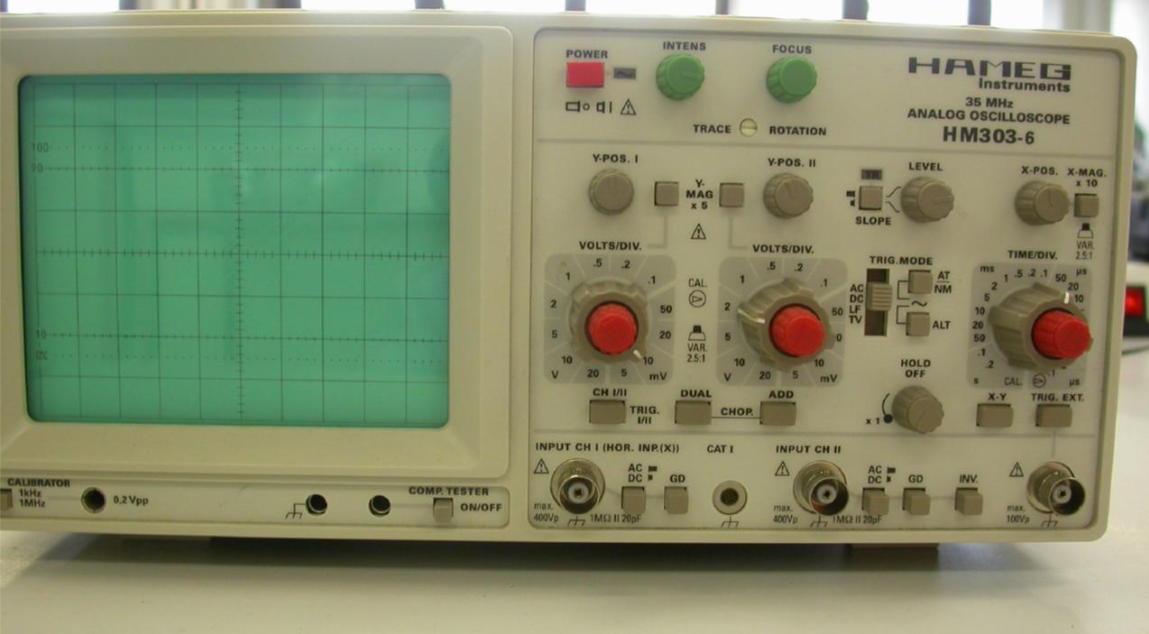
\includegraphics[width=\linewidth]{images/oszilloskop.png}
		\caption{Oszilloskop\cite{V300}}
		\label{fig:oszilloskop}
	\end{minipage}
\end{figure}
\begin{itemize}
	\item \textbf{Strahleinstellung (\texttt{POWER}, \texttt{INTEN}, \texttt{FOCUS}):} Über den Netzschalter \texttt{POWER} wird das Gerät eingeschaltet, mit den Reglern \texttt{INTEN} und \texttt{FOCUS} lassen sich Helligkeit und Schärfe des Elektronenstrahls einstellen.\cite{V300}
	\item \textbf{Vertikalablenkung (\texttt{V/DIV}, \texttt{Y-POS}):} Mit dem Stufenschalter \texttt{V/DIV} wird der vertikale Abbildungsmaßstab (\textit{Spannung pro Division}) für jeden Kanal getrennt gewählt, um die Amplitude an die Bildschirmhöhe anzupassen. Der innere rote Drehknopf dient zur Feinkalibrierung. Über \texttt{Y-POS\,I} bzw.\ \texttt{Y-POS\,II} lässt sich die Signallinie vertikal verschieben.\cite{V300}
	
	\item \textbf{Signalkopplung (\texttt{DC}, \texttt{AC}, \texttt{GD}):} Die Kopplungsschalter oberhalb der Eingangsbuchsen legen fest, wie das Eingangssignal an den Vertikalverstärker weitergeleitet wird\cite{V300}:
	\begin{itemize}
		\item \texttt{DC} (\textit{Direct Current}): Gleich- und Wechselspannungsanteil des Signals werden unverändert dargestellt. \cite{V300}
		\item \texttt{AC} (\textit{Alternating Current}): Der Gleichspannungsanteil wird blockiert, sodass ausschließlich überlagerte Wechselspannungsanteile (wie etwa der \textit{Ripple} nach einem Gleichrichter) bei hoher Empfindlichkeit sichtbar werden. \cite{V300}
		\item \texttt{GD} (\textit{Ground}): Der Verstärkereingang wird vom Messsignal getrennt und intern geerdet ($0\,\text{V}$) wird, um vor Gleichspannungsmessungen die Null-Referenzlinie auf dem Raster zu anzupassen. \cite{V300}
	\end{itemize}
	
	\item \textbf{Horizontalablenkung (\texttt{TIME/DIV}, \texttt{X-POS}, \texttt{X-MAG\,x10}):} Der Drehschalter \texttt{TIME/DIV} bestimmt die horizontale Ablenkgeschwindigkeit (Zeit pro \textit{Division}), die für beide Kanäle gleichermaßen gilt. Der zugehörige rote Innenregler ermöglicht den zeitlichen Feinabgleich bei der Kalibrierung. Mit \texttt{X-POS} wird das Signal horizontal verschoben. \cite{V300}
	
	\item \textbf{Trigger-Einheit (\texttt{LEVEL}, \texttt{SLOPE}, \texttt{TRIG.\,MODE}, \texttt{TRIG.\,I/II}):} Der Trigger synchronisiert den Startzeitpunkt der horizontalen Strahlablenkung mit dem periodischen Eingangssignal, sodass ein stehendes Bild entsteht. Mit \texttt{LEVEL} wird der Spannungsschwellenwert eingestellt, bei dessen Über- oder Unterschreiten die Ablenkung ausgelöst wird. Die Taste \texttt{SLOPE} wählt aus, ob auf die steigende (positive) oder fallende (negative) Signalflanke getriggert wird. Über \texttt{TRIG.\,I/II} wird die Triggerquelle festgelegt und über \texttt{TRIG.\,MODE} die Kopplungsart (\texttt{AC}/\texttt{DC}) des Triggersignals gewählt. \cite{V300}
	
	\item \textbf{Kalibrator (\texttt{CALIBRATOR}):} Die Ausgangsbuchse an der unteren linken Frontseite liefert ein internes Rechteck-Referenzsignal mit definierter Peak-to-Peak-Spannung ($0{,}2\,\text{V}_{\text{PP}}$) und fester Frequenz, mit dem Tastkopf und Kanalregler vor Versuchsbeginn abgeglichen werden. \cite{V300}
	
	
\end{itemize}

\subsection{Aufbau der Leiterplatte}

\begin{wrapfigure}{r}{0.4\textwidth}
	\centering
	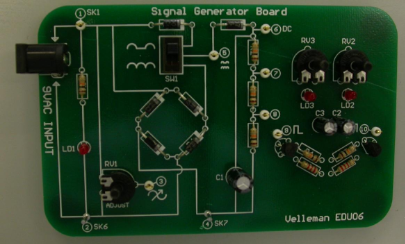
\includegraphics[width=\linewidth]{images/leiterplatte.png}
	\caption{Aufbau der Leiterplatte\cite{V300}}
	\label{fig:platte}
\end{wrapfigure}

Die vorliegende Leiterplatte (namentlich \enquote{Signal Generator Board}) besteht aus den Abgriffen \Circled{1} bis \Circled{10}, Potentiometern RV1 bis RV3, einem Schalter SW1 zum Wechseln zwischen Einweggleichrichter und Zweiweggleichrichter sowie Widerständen an unterschiedlichen Stellen, wie in \autoref{fig:platte} zu sehen.
Die Abgriffe \Circled{2} und \Circled{4} dienen hier als Erdungspunkte, an denen die Erdungsklemme befestigt werden kann.
Es ist möglich, mithilfe des Potentiometers RV1 das ausgehende Sinussignal an \Circled{3} zu verstellen. Weiterhin werden über RV2 und RV3 jeweils die Frequenz und das Puls-Pause-Verhältnis an den Abgriffen \Circled{9} und \Circled{10} angepasst.
Die Leiterplatte wird über einen Eingang mit einem Wechselstrom von $9\unit{\volt}$ AC betrieben (siehe \autoref{fig:platte} links).\cite{V300}

\subsection{Versuchsdurchführung}

Zuerst wird die Kalibrierung des Oszilloskops durchgeführt. Die Leiterplatte wird hierfür nicht verwendet. Es werden die Messspitze des Tastkopfes auf der Teilereinstellung x1 mit dem Abgriff $0.2\unit{\volt}_{PP}$ des Oszilloskops und die Erdungsklammer an einer Klemme der zwei Eingangsbuchsen am Oszilloskop verbunden. Über die Einstellung des zeitlichen Kanalreglers wird die Darstellung des Spannungsverlaufs angepasst, bis es statisch erscheint. Die Spannungshöhe wird nun mit Grobeinstellung und Feinjustierung angepasst, bis die Peak-to-Peak-Amplitude $U_{PP}$ mit den $0,2\unit{\volt}$ des Abgriffs $0.2\unit{\volt}_{PP}$ übereinstimmt. Zuletzt wird die Feinanpassung der Zeitachse anhand der am Oszilloskop eingestellten Kalibrierungsfrequenz durchgeführt. Die Feineinstellungen werden nach Vollendung der Kalibrierung beibehalten.

\subsubsection{Messung einer Sinusschwingung mit fester Frequenz}

Im Folgenden wird die Sinusschwingung einer festen Frequenz gemessen. Dazu wird die Messspitze des Tastkopfes an \Circled{1} angeschlossen und an \Circled{2} geerdet. Die Darstellung des Spannungsverlaufs wird wieder angepasst, bis es statisch erscheint. Der Versuch wird dreimal bei unterschiedlichen Einstellungen des Reglers V/DIV wiederholt. Es werden dazu Amplitude und Periode der Darstellung entnommen und daraus die Frequenz $v$

\begin{equation}
	v = \frac{1}{T}
\end{equation}

errechnet.\cite{V300}

\subsubsection{Messung einer Sinusschwingung mit variabler Amplitude}

Zur Vermessung der Sinusschwingung unter einer veränderbaren Amplitude wird der Abgriff \Circled{3} verwendet, der mit dem Potentiometer RV1 verbunden ist. Die Messspitze des Tastkopfes wird an \Circled{3} angebracht und die Erdungsklemme wird an \Circled{2} geklemmt. Es soll durch Drehen von RV1 die minimale sowie maximal erreichbare Amplitude von $U_{PP}$ gemessen werden. Im Anschluss wird dies mit dem Anschalten des Spannungsteilers auf $\frac{1}{10}$ wiederholt.

\subsubsection{Der Gleichrichter}

Der Spannungsteiler wird nun ausgeschaltet und die Messspitze des Tastkopfes mit \Circled{5} verbunden. Der Tastkopf wird über den Abgriff \Circled{4} geerdet.
Jetzt muss der Schalter SW1 in die obere Position gebracht werden, damit der Einweggleichrichter aktiv ist. Durch Umstellen der Kanalregler werden nun drei Halbwellen auf dem Oszilloskop dargestellt. Sobald dies erreicht ist, werden die Einstellungen der Kanalregler festgehalten. Mittels des Triggers wird die positive und negative Flanke ausgelöst, die dann skizziert werden.

Nun wird zu dem Zweiweggleichrichter gewechselt, indem der Schalter SW1 in die untere Position geschaltet wird. Es werden wieder relevante Einstellungen notiert und positive sowie negative Flanke skizziert.

\subsubsection{Gleichstrommessung}

Zur Messung wird die Messspitze des Tastkopfes zuerst mit dem Abgriff \Circled{6} verbunden, während weiterhin an \Circled{4} geerdet wird. Hierbei wird der Schalter SW1 auf die obere Stellung auf den Einweggleichrichter gestellt, Trigger Mode auf DC geschaltet und der Kanal durch Drücken von GD (Ground) geerdet. Die erkennbare Linie soll auf $0\unit{\volt}$ verlaufen. Jetzt wird durch Drücken von GD die entstandene vertikale Auslenkung gemessen. Daraufhin wird die Messung wiederholt, indem die Messspitze des Tastkopfes mit \Circled{7} und \Circled{8} nacheinander verbunden wird.

Nun wird die Messspitze des Tastkopfes wieder mit \Circled{6} verbunden. Die Erdungsklemme bleibt an \Circled{4}. Es wird der Trigger Mode auf AC geschaltet, wodurch ein \enquote{Ripple} messbar werden sollte, dessen Amplitude gemessen wird. Durch Umschalten von SW1 auf den Zweiweggleichrichter wird ein unterschiedlicher \enquote{Ripple} gemessen und beide werden verglichen.

\subsubsection{Signal mit variabler Frequenz}

Zuletzt wird ein Signal mit einer veränderbaren Frequenz vermessen. Dazu wird die Messspitze des Tastkopfes mit Abgriff \Circled{9} verbunden, geerdet wird über Abgriff \Circled{4}.
Nun sind Frequenz und Puls-Pause-Verhältnis je über RV2 und RV3 veränderbar. Es sollen die Anstiegszeiten der positiven und negativen Flanke abgemessen werden, sowie die Einstellungen des Kanalreglers notiert und die dargestellten Pulsformen skizziert werden.